\documentclass{scrartcl}

\RequirePackage[margin=1cm]{geometry}
\usepackage{amsmath}
\usepackage{pgfplots}

% Settings
\pgfplotsset{
  compat = 1.9,
  % ticks
  % ---------------------------------------
  every tick label/.append style={
    font=\small,
    align=center,
  },
  % labels
  % ---------------------------------------
  every axis/.append style={
    label style={font=\small, inner sep=0pt, outer sep=0pt},
  },
  xlabel near ticks,
  ylabel near ticks,
  xlabel={values},
  ylabel={P},
  % grids
  % ---------------------------------------
  grid = major,
  % legend
  % ---------------------------------------
  %legend pos=outer  north east,  
  every legend/.append style = {text=black,font=\small},
  % domain
  % ---------------------------------------
  % xmin=0, xmax=10,
  % ymin=0, ymax=0.5,
  % scale only axis,
}


\pgfplotscreateplotcyclelist{plotcolors}{%
  {sec_gray_dark,mark options={draw=prim_blue},mark=o},% map
  {sec_gray_dark,mark options={fill=prim_blue, draw=none},mark=*},% 1. client
  {sec_gray_dark,mark options={draw=prim_blue},mark=o},% 1. peers
  {sec_gray_dark,mark options={fill=ext_red},mark=square*},% 2. client
  {sec_gray_dark,mark options={draw=ext_red},mark=square},% 2. peers
  {sec_gray_dark,mark options={draw=ext_teal},mark=triangle},%
  {sec_gray_dark,mark options={draw=ext_navy},mark=pentagon},%
  {sec_gray_dark,mark options={draw=emph_green},mark=+},%
  {sec_gray_dark,mark options={draw=prim_blue},mark=x},%
}



% many plots: http://www.leg.ufpr.br/~walmes/tikz/


\begin{document}


\tikzset{
  declare function={ 
  	gamma(\z) =
    	(2.506628274631*sqrt(1/\z)+0.20888568*(1/\z)^(1.5)+
    	0.00870357*(1/\z)^(2.5)-(174.2106599*(1/\z)^(3.5))/25920-
    	(715.6423511*(1/\z)^(4.5))/1244160)*exp((-ln(1/\z)-1)*\z);
  },
  declare function={
    binom(\n,\x) = (\n!)/(\x!*(\n-\x)!);
  },
  declare function={
    binompf(\k,\n,\p)=\n!/(\k!*(\n-\k)!)*\p^\k*(1-\p)^(\n-\k);
  },
  declare function={
  	normal(\x,\mu,\sigma)=1/(\sigma*sqrt(2*pi))*exp(-((\x-\mu)^2)/(2*\sigma^2));
  },
}




\pgfmathdeclarefunction{gauss}{2}{%
  \pgfmathparse{1/(#2*sqrt(2*pi))*exp(-((x-#1)^2)/(2*#2^2))}%
}



\subsection{Uniform}

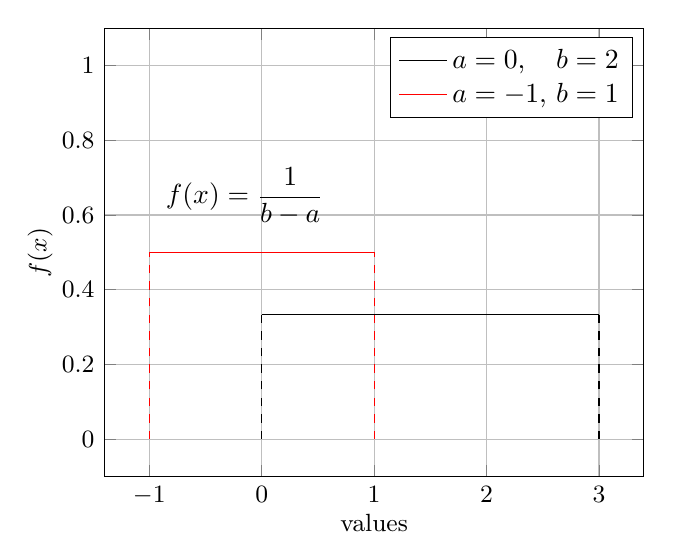
\begin{tikzpicture}[
  declare function={
    unifpdf(\x,\a,\b) = 1/(\b-\a);
  },
  ]

  \begin{axis}[
    samples=10, domain=0:5, no marks,
    ymax=1.1, ymin=-0.1,
    ylabel=$f(x)$]

    \addplot[smooth, domain=0:3]
    {unifpdf(x,0,3)};
    \addlegendentry{$a=0$, $\hphantom{-}b=2$};

    \addplot[smooth, domain=-1:1, color=red]
    {unifpdf(x,-1,1)};
    \addlegendentry{$a=-1$, $b=1$};

    \addplot[ycomb, mark=o, samples at={0,3}, dashed]
    {unifpdf(x,0,3)};
    \addplot[ycomb, mark=o, samples at={-1,1}, dashed, color=red]
    {unifpdf(x,-1,1)};

    \node at (axis cs: -0.15,  0.65)
    {$f(x) = \displaystyle \frac{1}{b-a}$};

  \end{axis}


\end{tikzpicture}






\subsection{Binomial}
\begin{tikzpicture}[
  hplot/.style={ycomb, mark=o}]

  \begin{axis}[
    width=10cm, height=6cm,
    xlabel=$x$, ylabel=$p(x)$,
    xlabel style={at={(1,0)}, anchor=north west},
    ylabel style={rotate=-90, at={(0,1)}, anchor=south east},
    legend style={draw=none, fill=none, font=\footnotesize},
    legend cell align=left,
    ymax=0.45,
    samples at={0,1,...,30},
    yticklabel style={
      /pgf/number format/fixed,
      /pgf/number format/fixed zerofill,
      /pgf/number format/precision=1
    }]

    \addplot[hplot] {binompf(x, 30, 0.3)};
    \addlegendentry{$n=30$, $p=0.3$}

    \addplot[hplot, red] {binompf(x, 30, 0.7)};
    \addlegendentry{$n=30$, $p=0.7$}

    \addplot[hplot, green] {binompf(x, 30, 0.9)};
    \addlegendentry{$n=30$, $p=0.9$}

    \addplot[hplot, blue, samples at={0,1,...,10}]
    {binompf(x, 10, 0.3)};
    \addlegendentry{$n=10$, $p=0.3$}

    \node at (axis description cs: 0.33, 0.8)
    {$p(x) = \binom{n}{p}\cdot p^x \cdot (1-p)^{n-x} $};

  \end{axis}
\end{tikzpicture}



\subsection{Negative Binomial}
\begin{tikzpicture}[
  declare function={
    bnegpf(\k,\p,\r)=(binom(\k-1, \r-1))*\p^(\r)*(1-\p)^(\k-\r);
  },
  hplot/.style={ycomb, mark=o}]

  \begin{axis}[
    width=10cm, height=6cm,
    xlabel=$x$, ylabel=$p(x)$,
    xlabel style={at={(1,0)}, anchor=north west},
    ylabel style={rotate=-90, at={(0,1)}, anchor=south east},
    legend style={draw=none, fill=none, font=\footnotesize},
    legend cell align=left]

    \addplot[hplot, samples at={1,2,...,21}]
    {bnegpf(x, 0.5, 1)};
    \addlegendentry{$p=0.5$, $r=1$}

    \addplot[hplot, samples at={5,6,...,21}, red]
    {bnegpf(x, 0.5, 5)};
    \addlegendentry{$p=0.5$, $r=5$}

    \addplot[hplot, samples at={5,6,...,21}, blue]
    {bnegpf(x, 0.8, 5)};
    \addlegendentry{$p=0.8$, $r=5$}

    \node at (axis description cs: 0.65, 0.5)
    {$p(x) = \binom{x-1}{r-1} \cdot p^r \cdot (1-p)^{x-r}$};

  \end{axis}
\end{tikzpicture}




\subsection{Gauss}

\begin{tikzpicture}
\begin{axis}[
  no markers, domain=0:10, samples=100,
  axis lines*=left, xlabel=$x$, ylabel=$y$,
  every axis y label/.style={at=(current axis.above origin),anchor=south},
  every axis x label/.style={at=(current axis.right of origin),anchor=west},
  height=5cm, width=12cm,
  xtick={4,6.5}, ytick=\empty,
  enlargelimits=false, clip=false, axis on top,
  grid = major
  ]
  \addplot [fill=cyan!20, draw=none, domain=0:5.96] {normal(x,6.5,1)} \closedcycle;
  \addplot [very thick,cyan!50!black] {gauss(4,1)};
  \addplot [very thick,cyan!50!black] {gauss(6.5,1)};


\draw [yshift=-0.6cm, latex-latex](axis cs:4,0) -- node [fill=white] {$1.96\sigma$} (axis cs:5.96,0);
\end{axis}

\end{tikzpicture}






\subsection{Normal}

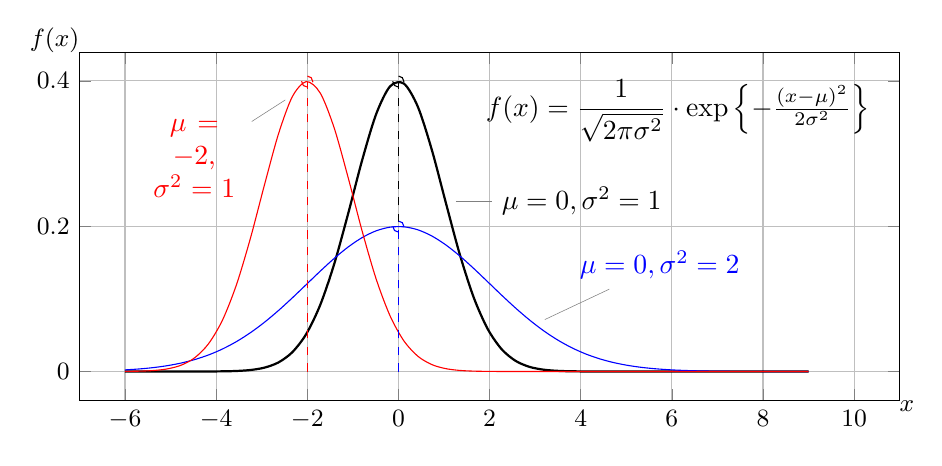
\begin{tikzpicture}[
  declare function={
    normalpdf(\x,\mu,\sigma)=
    (2*3.1415*\sigma^2)^(-0.5)*exp(-(\x-\mu)^2/(2*\sigma^2));
  },
  hplot/.style={ycomb, mark=o, dashed}]

  \begin{axis}[
    width=12cm, height=6cm,
    samples=50,
    xlabel=$x$, ylabel=$f(x)$,
    xlabel style={at={(1,0)}, anchor=north west},
    ylabel style={rotate=-90, at={(0,1)}, anchor=south east},
    legend style={draw=none, fill=none},
    domain=-6:9,
    legend cell align=left,
    xmin=-7, xmax=11]

    \addplot [smooth, thick] {normalpdf(x,0,1)}
    node[pos=0.47, pin={right:$\mu=0,\sigma^2=1$}] {};
    \addplot [smooth, blue] {normalpdf(x,0,2)}
    node[pos=0.6, pin={45:$\mu=0,\sigma^2=2$}] {};
    \addplot [smooth, red] {normalpdf(x,-2,1)}
    node[pos=0.25, pin={[text centered, text width=8ex]
      200:$\mu=-2$, $\sigma^2=1$}] {};

    \addplot [hplot, samples at={0}] {normalpdf(x,0,1)};
    \addplot [hplot, samples at={0}, blue] {normalpdf(x,0,2)};
    \addplot [hplot, samples at={-2}, red] {normalpdf(x,-2,1)};

    \node[anchor=north east] at (axis description cs: 0.975,  0.95)
    {$f(x) = \dfrac{1}{\sqrt{2\pi\sigma^2}}\cdot 
      \exp\left\{-\frac{(x-\mu)^2}{2\sigma^2}\right\}$};

  \end{axis}
\end{tikzpicture}








\subsection{Poisson}
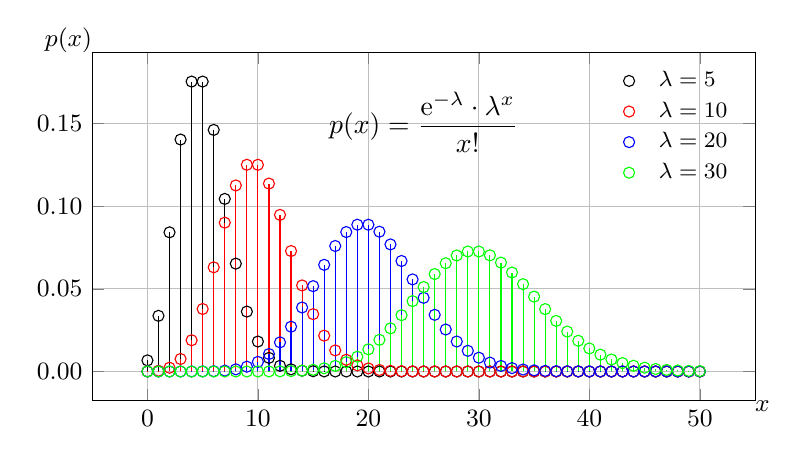
\begin{tikzpicture}[
  declare function={
    poispf(\k,\l) = exp(-\l)*(\l^\k)/(\k!);
  },
  hplot/.style={ycomb, mark=o}]

  \begin{axis}[
    width=10cm, height=6cm,
    xlabel=$x$, ylabel=$p(x)$,
    xlabel style={at={(1,0)}, anchor=north west},
    ylabel style={rotate=-90, at={(0,1)}, anchor=south east},
    legend style={draw=none, fill=none, font=\footnotesize},
    legend cell align=left,
    samples at={0,1,...,50},
    yticklabel style={
      /pgf/number format/fixed,
      /pgf/number format/fixed zerofill,
      % /pgf/number format/precision=2
    }]

    \addplot[hplot, black] {poispf(x, 5)};
    \addlegendentry{$\lambda=5$}
    \addplot[hplot, red] {poispf(x, 10)};
    \addlegendentry{$\lambda=10$}
    \addplot[hplot, blue] {poispf(x, 20)};
    \addlegendentry{$\lambda=20$}
    \addplot[hplot, green] {poispf(x, 30)};
    \addlegendentry{$\lambda=30$}

    \node at (axis description cs: 0.5, 0.8)
    {$p(x) = \dfrac{\text{e}^{-\lambda}\cdot \lambda^x}{x!}$};

  \end{axis}
\end{tikzpicture}






\subsection{Hypergeometric}

\begin{tikzpicture}[
  declare function={
    hiperpf(\x,\N,\n,\K) = binom(\K, \x)*binom(\N-\K, \n-\x)/binom(\N, \n);
  },
  hplot/.style={ycomb, mark=o}]

  \begin{axis}[
    width=10cm, height=6cm,
    xlabel=$x$, ylabel=$p(x)$,
    xlabel style={at={(1,0)}, anchor=north west},
    ylabel style={rotate=-90, at={(0,1)}, anchor=south east},
    legend style={draw=none, fill=none, font=\footnotesize},
    legend cell align=left,
    xtick={0,1,...,10},
    ymax=0.75]

    \addplot[hplot, samples at={0,1,...,10}]
    (x, {hiperpf(x, 20, 10, 10)});
    \addlegendentry{$N=20$, $n=10$, $K=10$}

    \addplot[hplot, samples at={0,1,...,10}, red]
    (x-0.1, {hiperpf(x, 50, 10, 25)});
    \addlegendentry{$N=50$, $n=10$, $K=25$}

    \addplot[hplot, samples at={0,1,...,5}, blue]
    (x+0.1, {hiperpf(x, 50, 10, 5)});
    \addlegendentry{$N=50$, $n=10$, $K=5$}

    \node[anchor=north] at (axis description cs: 0.25, 0.95)
    {$p(x) = \dfrac{\binom{K}{x} \binom{N-k}{n-x}}{\binom{N}{n}}$};

  \end{axis}
\end{tikzpicture}







\subsection{Exponential}

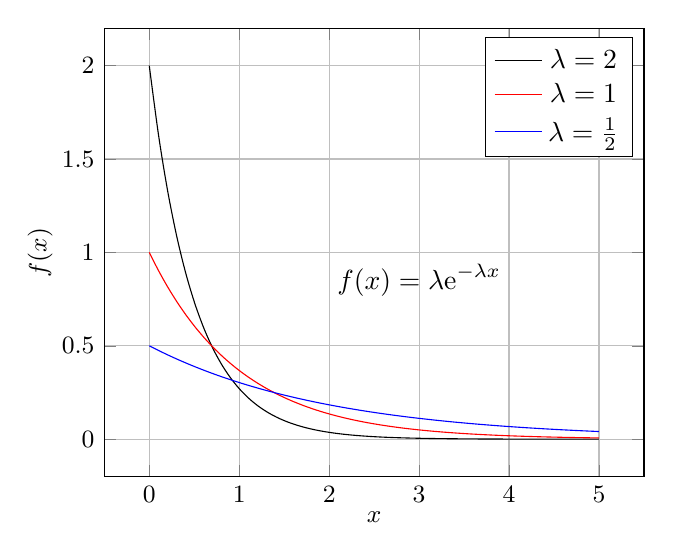
\begin{tikzpicture}[
  declare function={
    exppdf(\x,\lambda) = \lambda*exp(-\lambda*\x);
  },
  ]

  \begin{axis}[
  		samples=50, domain=0:5, smooth, no marks,
  		xlabel=$x$,
  		ylabel=$f(x)$
  	]
    \addplot[color=black] {exppdf(x,2)};
    \addlegendentry{$\lambda=2$};
    \addplot[color=red] {exppdf(x,1)};
    \addlegendentry{$\lambda=1$};
    \addplot[color=blue] {exppdf(x,0.5)};
    \addlegendentry{$\lambda=\frac{1}{2}$};
    \node[rotate=0] at (axis cs: 3,  0.85)
    {$f(x) = \displaystyle \lambda \text{e}^{-\lambda x}$};
  \end{axis}

\end{tikzpicture}







\subsection{Gamma}


\begin{tikzpicture}[
    declare function={gammapdf(\x,\k,\theta) = \x^(\k-1)*exp(-\x/\theta) / (\theta^\k*gamma(\k));}
]

\begin{axis}[
    axis lines=left,
    enlargelimits=upper,
    samples=50,
    legend entries={$k=1\quad \theta=2$,$k=2\quad \theta=2$, $k=9\quad \theta=0.5$}
]
\addplot [smooth, domain=0:20] {gammapdf(x,1,2)};
\addplot [smooth, domain=0:20, red] {gammapdf(x,2,2)};
\addplot [smooth, domain=0:20, blue] {gammapdf(x,9,0.5)};
\end{axis}
\end{tikzpicture}






\subsection{Beta}

\begin{tikzpicture}[
  declare function={
    beta(\a,\b) = gamma(\a)*gamma(\b)/gamma(\a+\b);
  },
  declare function={
    betapdf(\x,\a,\b) = \x^(\a-1)*(1-\x)^(\b-1)/beta(\a,\b);
  }]

  \begin{axis}[
    width=9cm, height=6cm,
    samples=30,
    xlabel=$x$, ylabel=$f(x)$,
    xlabel style={at={(1,0)}, anchor=north west},
    ylabel style={rotate=-90, at={(0,1)}, anchor=south east},
    legend style={draw=none, fill=none},
    domain=0.01:0.99,
    legend pos=outer north east,
    legend cell align=left,
    clip=false]

    \addplot[smooth] {betapdf(x,1,1)};
    \addlegendentry{$\alpha=1$, $\phantom{.}\beta=1$};

    \addplot[smooth, red] {betapdf(x,5,5)};
    \addlegendentry{$\alpha=5$, $\phantom{.}\beta=5$};

    \addplot[smooth, blue] {betapdf(x,.7,.7)};
    \addlegendentry{$\alpha=.7$, $\beta=.7$};

    \addplot[smooth, orange] {betapdf(x,.7,1.2)};
    \addlegendentry{$\alpha=.7$, $\beta=1.2$};

    \addplot[smooth, purple] {betapdf(x,5,2)};
    \addlegendentry{$\alpha=5$, $\phantom{.}\beta=2$};

    \node[anchor=west] at (axis description cs: 1.05, 0.2)
    {$f(x) = \dfrac{x^{\alpha-1}\cdot(1-x)^{\beta-1}}{
        B(\alpha, \beta)}$};

  \end{axis}
\end{tikzpicture}



\end{document}
